\chapter{Лабораторная работа №6. Цифровая обработка сигналов}

\section{Арифметика с плавающей точкой}

\begin{figure}[h]
	\centering
	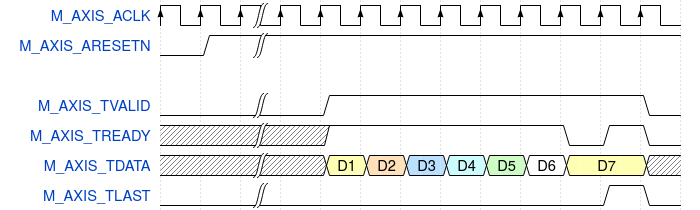
\includegraphics[width=0.9\textwidth]{image/axis_0.png}
	\caption{Временная диаграмма работы интерфейса AXI4-Stream}
	\label{axis}
\end{figure}

AXI4-Stream — это протокол, предназначенный для передачи однонаправленных данных(см.рис.~\ref{axis}). В AXI4-Stream биты ширины TDATA передаются за такт. Передача начинается, когда ведущее устройство(master) отправляет сигнал TVALID, а ведомое устройство(slave) отвечает, отправляя сигнал TREADY(этот механизм был рассмотрен выше, при рассмотрении интерфейса AXI4-Lite). В этот момент мастер начнет отправлять TDATA и TLAST (TUSER, если необходимо передать дополнительные данные, определяемые пользователем). TLAST сигнализирует о последнем слове потока. Таким образом, ведомое устройство(slave) продолжает потреблять входящие TDATA до тех пор, пока TLAST не будет установлен.

\begin{figure}[h]
	\centering
	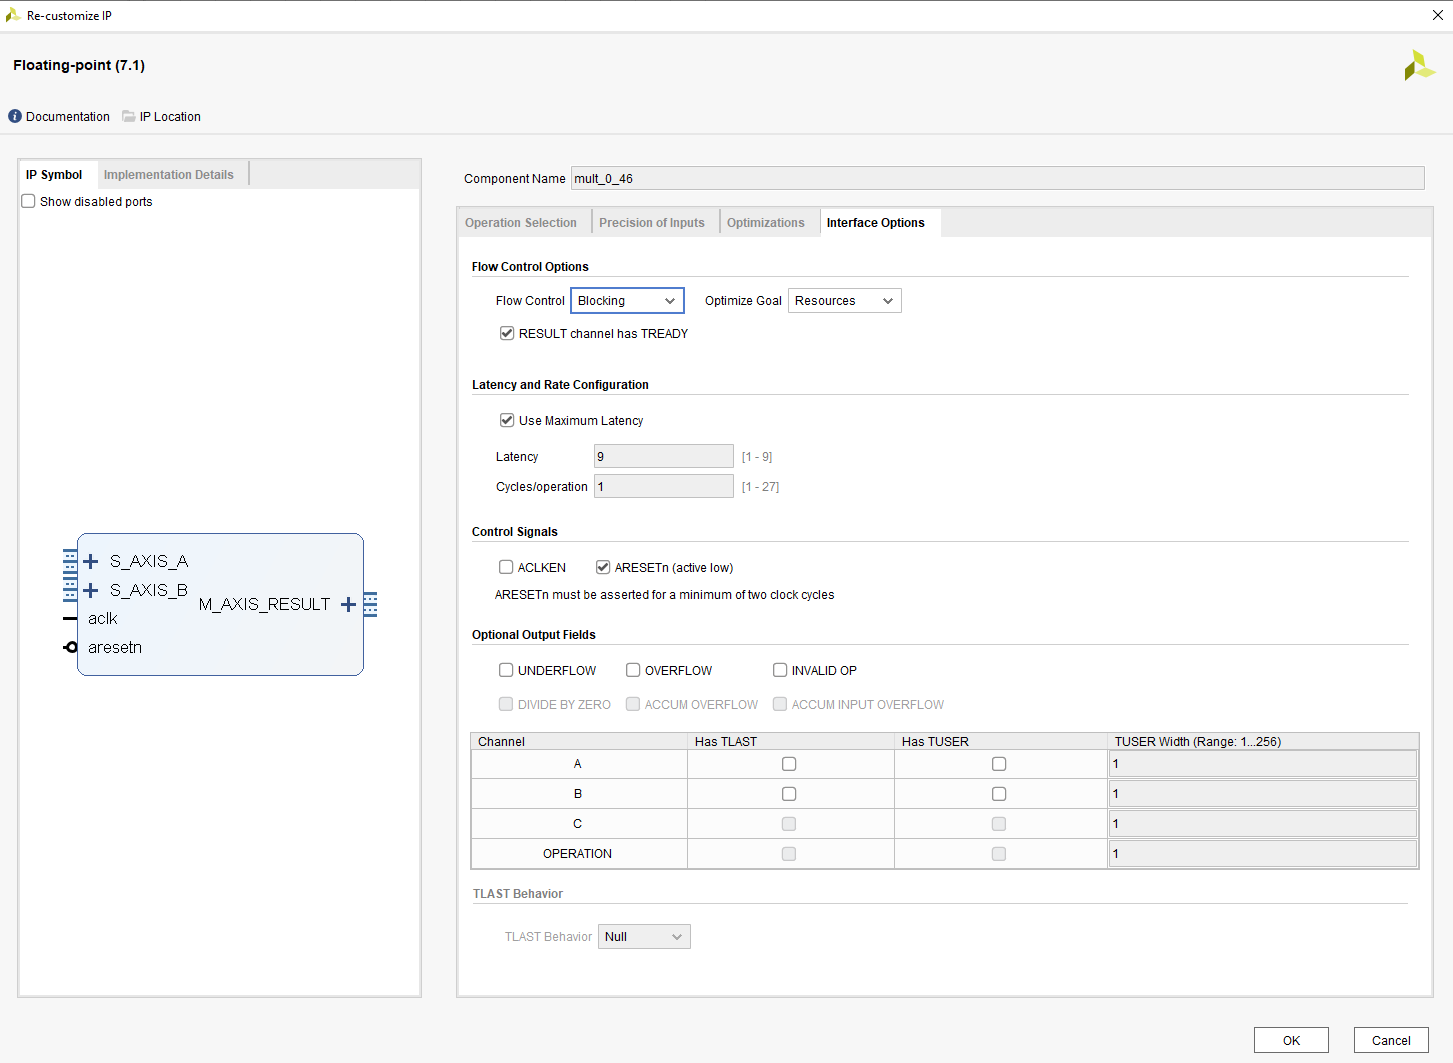
\includegraphics[width=0.5\textwidth]{image/fp_interface_options.png}
	\caption{Временная диаграмма работы интерфейса AXI4-Stream}
	\label{fp_interface_options}
\end{figure}

\begin{figure}[h]
	\centering
	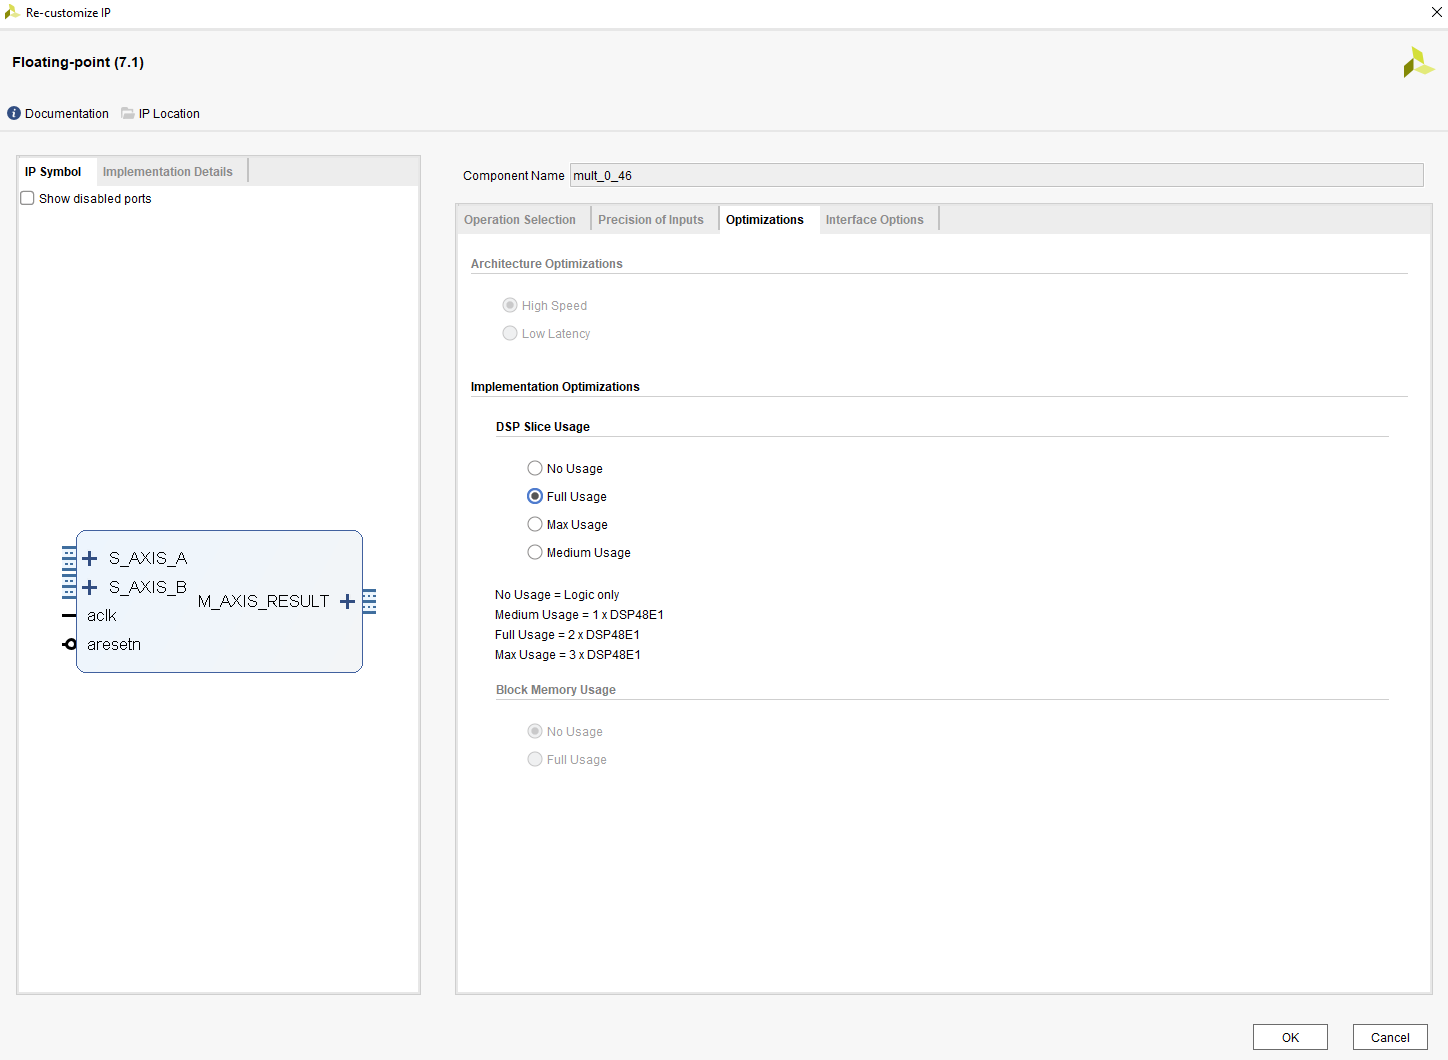
\includegraphics[width=0.5\textwidth]{image/fp_optimizations.png}
	\caption{Временная диаграмма работы интерфейса AXI4-Stream}
	\label{fp_optimizations}
\end{figure}

\begin{figure}[h]
	\centering
	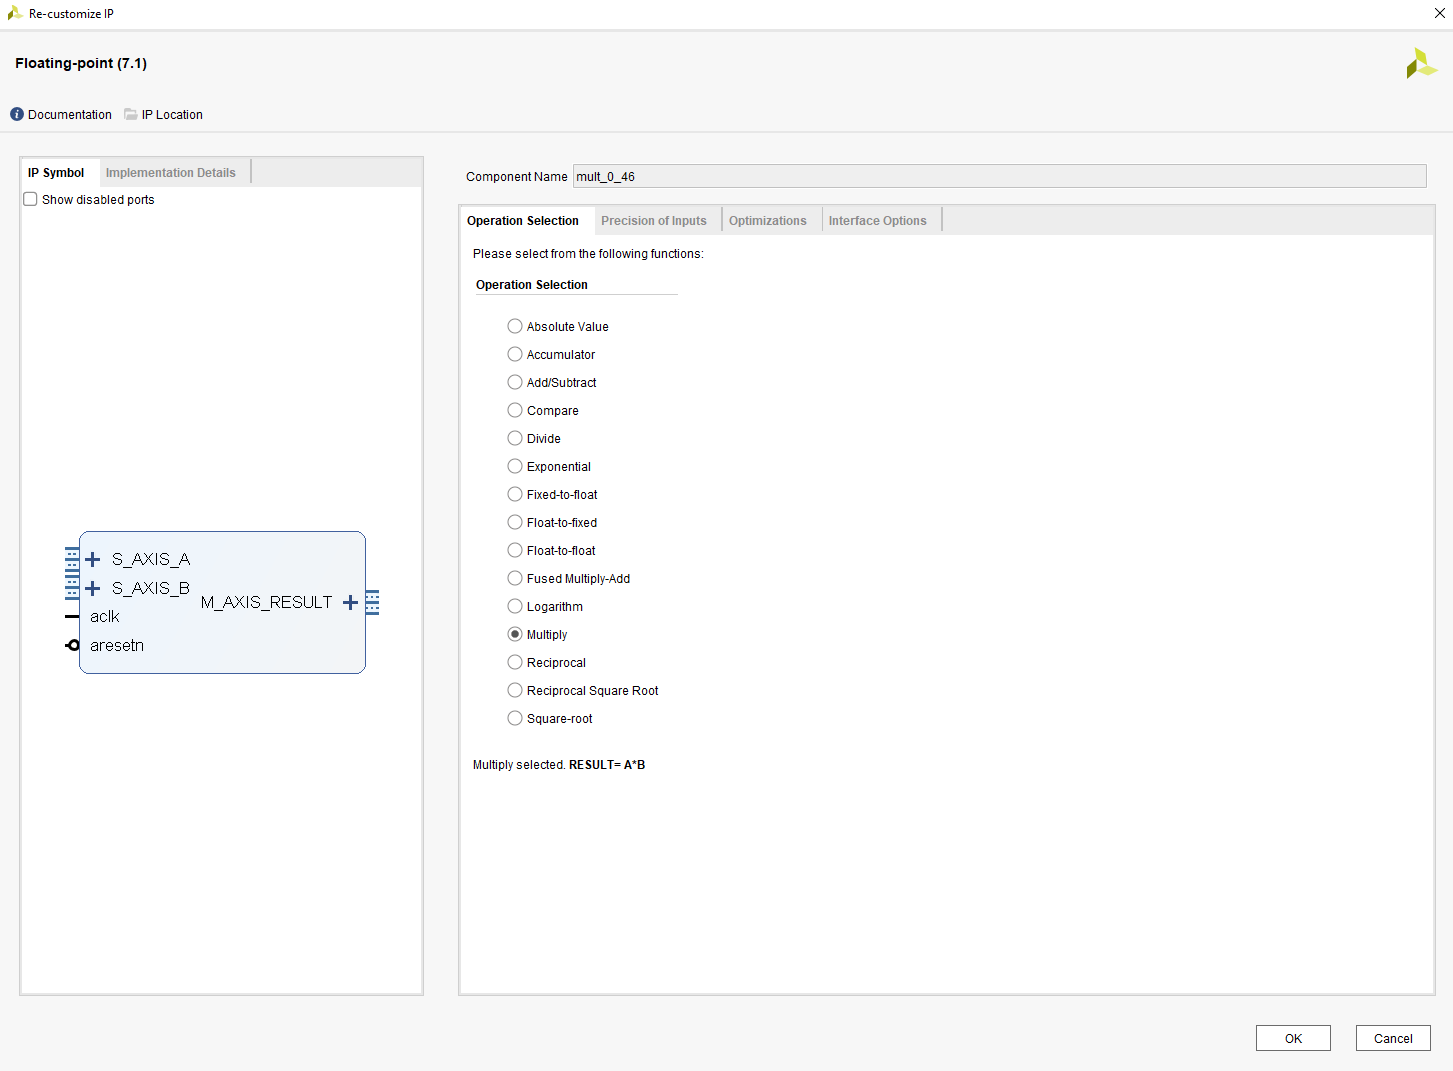
\includegraphics[width=0.5\textwidth]{image/fp_selection_tab.png}
	\caption{Временная диаграмма работы интерфейса AXI4-Stream}
	\label{fp_selection_tab}
\end{figure}

\begin{figure}[h]
	\centering
	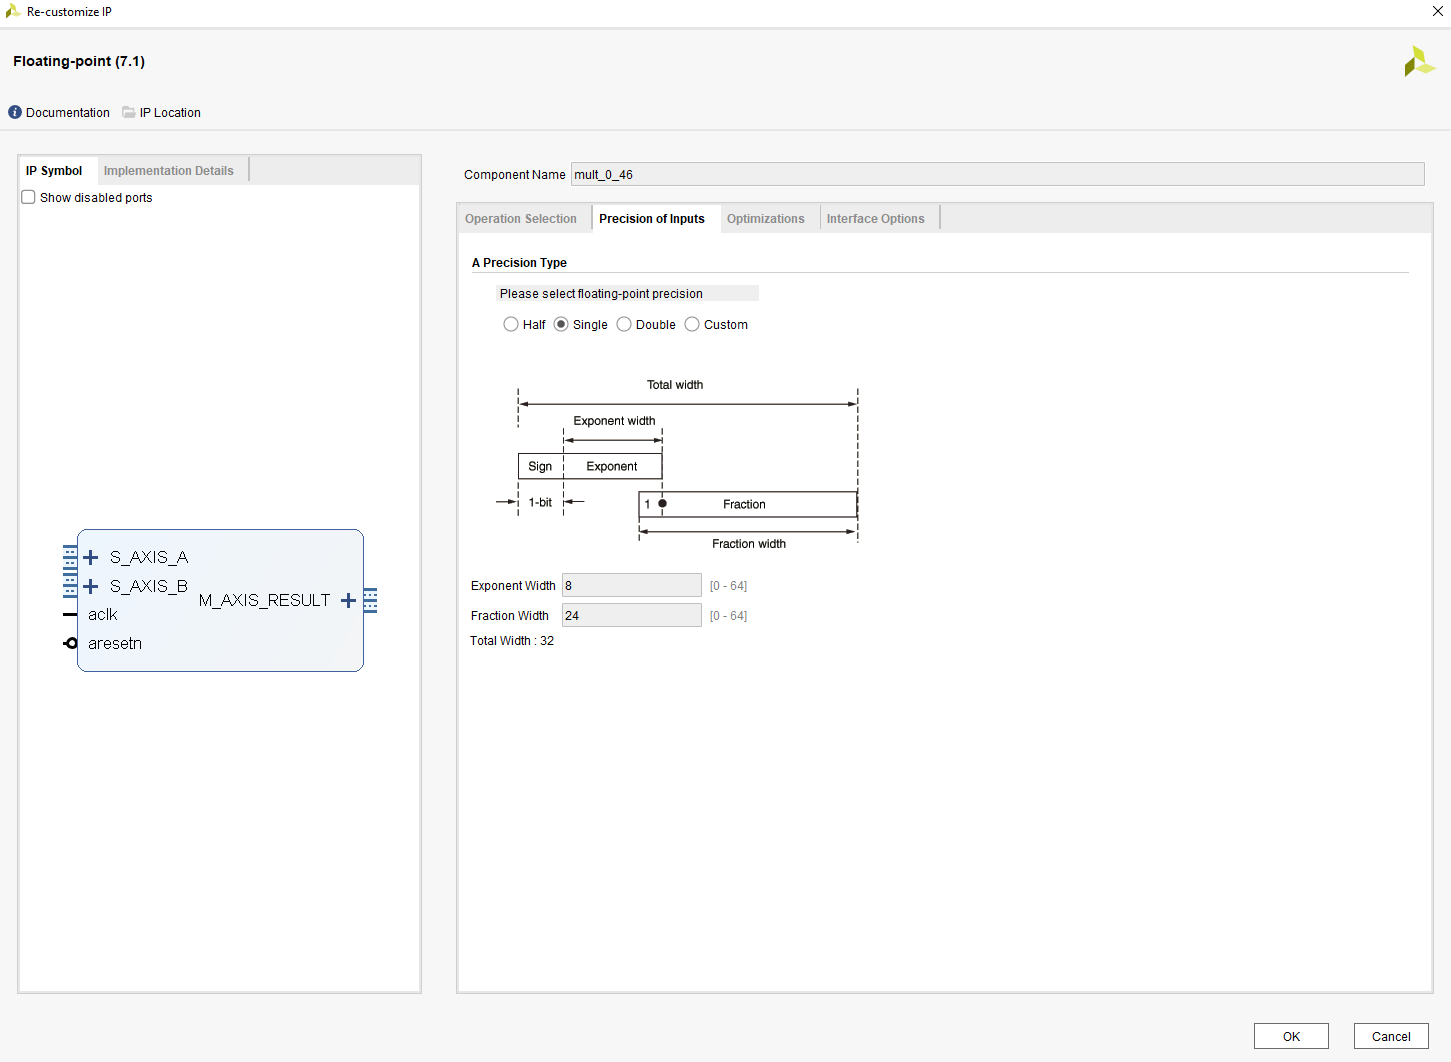
\includegraphics[width=0.5\textwidth]{image/fp_precision_type.png}
	\caption{Временная диаграмма работы интерфейса AXI4-Stream}
	\label{fp_precision_type}
\end{figure}

\section{Быстрое преобразование Фурье}
	Выражение для дискретного преобразования Фурье имеет следующий вид:

\begin{align*}
f[k] &= \sum_{j=0}^{N-1} x[j]\left(e^{-2\pi i k/N}\right)^j\\
0 &\leq k < N
\end{align*}

\begin{figure}[h]
    \centering
    \noindent
	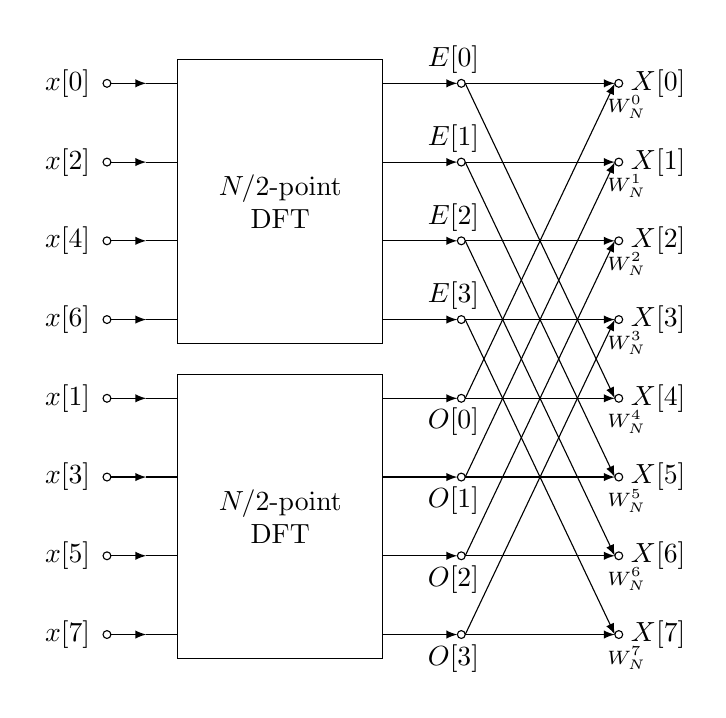
\begin{tikzpicture}% Example:
	  \draw[fill=white, draw=white] (-0.5, 0.7) rectangle (8, -7.7); 
	  \draw (0,0) node {$x[0]$};
	  \draw (0,-1) node {$x[2]$} ;
	  \draw (0,-2) node {$x[4]$} ;
	  \draw (0,-3) node {$x[6]$} ;
	
	  \draw (0,-4) node {$x[1]$} ;
	  \draw (0,-5) node {$x[3]$} ;
	  \draw (0,-6) node {$x[5]$} ;
	  \draw (0,-7) node {$x[7]$} ;
	
	  % arrow on the right of x's
	  \foreach \n in {0,...,7} {
	    \draw (0.5,-\n) circle(0.05)[fill=white]; 
	    \draw [-latex] (0.55,-\n) -- (1, -\n); 
	    \draw (1, -\n) -- (1.4, -\n); 
	  }
	
	  % blocks
	  \draw(1.4, 0.3) rectangle (4, -3.3); 
	  \draw(1.4, -3.7) rectangle (4, -7.3); 
	  \draw(2.7, -1.5) node[text centered, text width=2cm] {$N/2$-point DFT};
	  \draw(2.7, -5.5) node[text centered, text width=2cm] {$N/2$-point DFT};
	
	  % E's and O's 
	  \foreach \n in {0,...,7} {
	    \draw [-latex] (4,-\n) -- (4.95, -\n); 
	    \draw (5,-\n) circle(0.05)[fill=white]; 
	  }
	  \foreach \n in {0,...,3} {
	    \draw (4.9,-\n + 0.3) node {$E[\n]$};
	  }
	  \foreach \n in {0,...,3} {
	    \draw (4.9,-\n - 4 - 0.3) node {$O[\n]$};
	  }
	
	  % X's 
	  \foreach \n in {0,...,7} {
	    \draw (7,-\n) circle(0.05)[fill=white]; 
	    \draw (7.5,-\n) node {$X[\n]$};
	  }
	
	  % Connecting X and E
	  \foreach \n in {0,...,7} {
	    \draw [-latex] (5.05, -\n) -- (6.95, -\n);
	  }
	  \foreach \n in {0,...,3} {
	    \draw [-latex] (5.05, -\n) -- (6.95, -\n - 4);
	  }
	  \foreach \n in {0,...,3} {
	    \draw [-latex] (5.05, -\n-4) -- (6.95, -\n);
	  }
	
	  % W's
	  \foreach \n in {0,...,7} {
	    \draw (7.1,-\n - 0.3) node {\scriptsize $W_N^{\n}$};
	  }
	\end{tikzpicture}
\end{figure}

\begin{figure}[h]
	\centering
	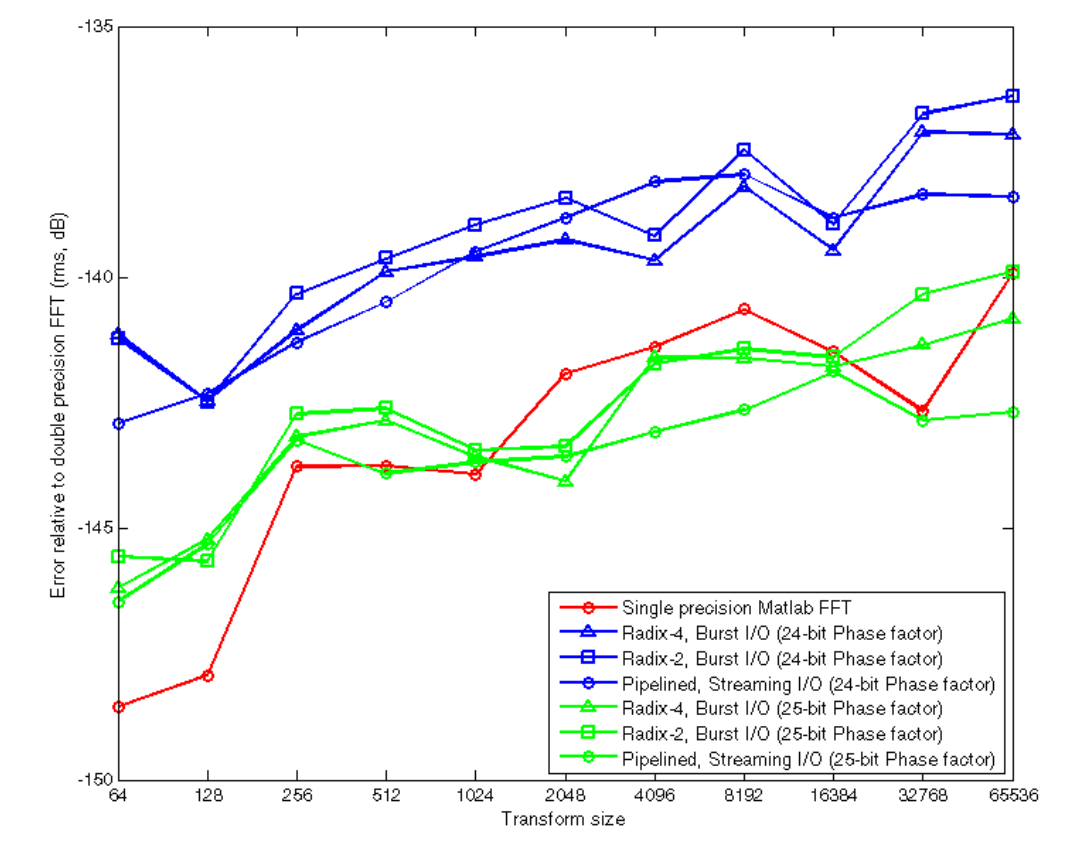
\includegraphics[width=0.5\textwidth]{image/fft_xilinx_fp.png}
	\caption{Временная диаграмма работы интерфейса AXI4-Stream}
	\label{fft_detailed_implem}
\end{figure}

Варианты архитектуры
Ядро БПФ предлагает четыре варианта архитектуры, обеспечивающие компромисс между размером ядра и временем преобразования. • Конвейерный потоковый ввод-вывод — обеспечивает непрерывную обработку данных. • Пакетный ввод-вывод Radix-4 — загружает и обрабатывает данные отдельно, используя итеративный подход. Оно меньше по размеру, чем конвейерное решение, но имеет большее время преобразования. • Пакетный ввод-вывод Radix-2 — использует тот же итеративный подход, что и Radix-4, но бабочка меньше. Это означает, что он меньше по размеру, чем решение Radix-4, но время преобразования больше. • Radix-2 Lite Burst I/O — основанный на архитектуре Radix-2, этот вариант использует подход с временным мультиплексированием к бабочке для еще меньшего ядра за счет более длительного времени преобразования. Рисунок 3-35 иллюстрирует компромисс между пропускной способностью и использованием ресурсов для четырех архитектур. Как правило, каждая архитектура предлагает двухкратную разницу в ресурсах по сравнению со следующей архитектурой. Пример для четной степени размера 2 пункта. Это не требует, чтобы архитектура Radix-4 имела дополнительную ступень Radix-2. Все четыре архитектуры могут быть настроены для использования интерфейса с фиксированной запятой с одним из трех арифметических методов с фиксированной запятой (немасштабированные, масштабированные или блочные с плавающей запятой) или могут вместо этого использовать интерфейс с плавающей запятой.

Прямой и реверсный порядок

Каждая архитектура предлагает возможность естественного или обратного упорядочения выходных данных, когда данные вводятся в естественном порядке. Алгоритм БПФ переупорядочивает выборки во время обработки таким образом, что данные, вводимые в естественном порядке, выводятся в обратном порядке. Ядро может опционально выводить данные в естественном порядке. Однако это налагает затраты на каждую архитектуру. Для архитектур Burst I/O это приводит к потере времени, поскольку выгрузка данных не может происходить одновременно с загрузкой входных данных для следующего кадра, поэтому требуются отдельные фазы выгрузки и загрузки. В конвейерной архитектуре для выполнения переупорядочения требуется дополнительная память ОЗУ. В архитектурах Radix-2 Burst I/O, Radix-2 Lite Burst I/O и Pipelined Streaming I/O обратный порядок битов легко вычислить, взяв индекс точки данных, записанный в двоичном виде, и реверсивное преобразование. порядок цифр. Следовательно, 0000, 0001, 0010, 0011, 0100,... (0, 1, 2, 3, 4,...) становятся 0000, 1000, 0100, 1100, 0010,... (0, 8, 4). , 12, 2,...).

В случае архитектуры пакетного ввода-вывода Radix-4 реверсирование применяется к цифрам и поэтому называется реверсированием цифр. Цифра в Radix-4 состоит из двух битов. Следовательно, 0000, 0001, 0010, 0011, 0100,... (0, 1, 2, 3, 4,...) становятся 0000, 0100, 1000, 1100, 0001,... (0, 4, 8). , 12, 1,...), поскольку пары цифр меняются местами. Если размер преобразования требует нечетного числа битов индекса, нечетная цифра из младшего разряда перемещается в старший разряд, поэтому 00000, 00001, 00010, 00011, 00100,... (0, 1, 2, 3 , 4,...) становится 00000, 10000, 00100, 10100, 01000,...(0, 16, 4, 20, 8,...)

Решение Pipelined Streaming I/O объединяет несколько механизмов обработки бабочки Radix-2 для обеспечения непрерывной обработки данных. Каждый механизм обработки имеет свои собственные банки памяти для хранения входных и промежуточных данных (рис. 3-36). Ядро имеет возможность одновременно выполнять вычисления преобразования для текущего фрейма данных, загружать входные данные для следующего фрейма данных и выгружать результаты предыдущего фрейма данных. Вы можете непрерывно передавать данные и, после задержки вычисления, можете непрерывно выгружать результаты. При желании этот дизайн также может вычислять один кадр сам по себе или кадры с промежутками между ними.

В масштабированном режиме фиксированной точки данные масштабируются после каждой пары этапов Radix-2. Блочный режим с плавающей запятой может использовать значительно больше ресурсов, чем режим масштабирования, поскольку он должен поддерживать дополнительные биты точности, чтобы обеспечить динамическое масштабирование без ущерба для производительности. Следовательно, если входные данные хорошо изучены и маловероятно, что они будут демонстрировать большие колебания амплитуды, достаточно использовать масштабированную арифметику (с подходящим графиком масштабирования, чтобы избежать переполнения в известном наихудшем случае), и ресурсы могут быть сохранены. Входные данные представлены в естественном порядке. Выгруженные выходные данные могут быть либо в обратном порядке битов, либо в естественном порядке. При выборе выходных данных естественного порядка используется дополнительный ресурс памяти. Эта архитектура охватывает размеры точек от 8 до 65536. У вас есть возможность выбрать количество этапов для использования блочной ОЗУ для хранения данных и фазового коэффициента. Остальные этапы используют распределенную память.

В решении Radix-4 Burst I/O ядро FFT использует один механизм обработки бабочки Radix-4 (рис. 3-37). Он загружает и/или выгружает данные отдельно от вычисления преобразования. Ввод/вывод данных и их обработка не являются одновременными. При запуске БПФ данные загружаются. После загрузки полного кадра ядро вычисляет преобразование. По завершении вычисления данные могут быть выгружены, но не могут быть загружены или выгружены в процессе вычисления. Процессы загрузки и выгрузки данных могут перекрываться, если данные выгружаются в обратном порядке цифр. Эта архитектура использует меньше ресурсов, чем архитектура конвейерного потокового ввода-вывода, но имеет более длительное время преобразования и поддерживает размеры точек от 64 до 65536. Данные и фазовые коэффициенты могут храниться в блочной ОЗУ или в распределенной ОЗУ (последняя для размеров точек). меньше или равно 1024).

В архитектуре ввода-вывода Radix-2 Burst используется один механизм обработки данных Radix-2 в виде бабочки (рис. 3-38). После загрузки кадра данных поток входных данных должен быть остановлен до завершения вычисления преобразования. Затем данные можно выгрузить. Как и в архитектуре Radix-4 Burst I/O, данные могут загружаться и выгружаться одновременно, когда выходные отсчеты находятся в обратном порядке битов. Это решение поддерживает размеры точек от 8 до 65536. Как память данных, так и память фазового коэффициента могут находиться либо в блочной ОЗУ, либо в распределенной ОЗУ (последняя для размеров точек меньше или равных 1024).

Эта архитектура отличается от Radix-2 Burst I/O тем, что механизм обработки данных типа «бабочка» использует один общий сумматор/вычитатель, тем самым сокращая ресурсы за счет дополнительной задержки на вычисление типа «бабочка». Опять же, как и в случае архитектур Burst I/O Radix-4 и Radix-2, данные могут быть одновременно загружены и выгружены только в том случае, если выходные отсчеты находятся в обратном порядке битов. Это решение поддерживает размеры точек от 8 до 65536. См. рис. 3-39.

\begin{enumerate}
	\item \verb|event_frame_started| Этот сигнал события устанавливается в течение одного тактового цикла, когда ядро начинает обрабатывать новый кадр. Этот сигнал предназначен для подсчета кадров и синхронизации конфигурации ядра с конкретным кадром, если это необходимо.
	\item \verb|event_tlast_missing|
	Этот сигнал события устанавливается в течение одного тактового цикла, когда \verb|s_axis_data_tlast| имеет значение Low для последней входящей выборки данных кадра. Это показывает несоответствие конфигурации между ядром и вышестоящим источником данных в отношении размера кадра и указывает, что вышестоящий источник данных настроен на больший размер точки, чем ядро. Это вычисляется только тогда, когда ядро начинает обработку кадра, поэтому событие может отставать от отсутствующего \verb|s_axis_data_tlast| на большое количество тактов.
	\item \verb|event_tlast_unexpected|
	Этот сигнал события утверждается в течение одного тактового цикла, когда ядро видит \verb|s_axis_data_tlast| High для любой входящей выборки данных, которая не является последней в кадре. Это показывает несоответствие конфигурации между ядром и восходящим источником данных в отношении размера кадра и указывает, что восходящий источник данных настроен на меньший размер точки, чем ядро. Это вычисляется только тогда, когда ядро начинает обработку кадра, поэтому событие может отставать от неожиданного High на \verb|s_axis_data_tlast| на большое количество тактовых циклов. Если на \verb|s_axis_data_tlast| для кадра есть несколько неожиданных максимумов, то это утверждается для каждого из них.
	\item \verb|event_fft_overflow|
	Этот сигнал о событии устанавливается в каждом тактовом цикле, когда наблюдается переполнение в выборках данных, передаваемых на \verb|m_axis_data_tdata|. Переполнение БПФ возможно только при использовании масштабированной арифметики или ввода-вывода с плавающей запятой одинарной точности. Во всех других конфигурациях штифт удаляется из сердечника.
	\item \verb|event_data_in_channel_halt|
	Это событие подтверждается в каждом цикле, когда ядру требуются данные из канала ввода данных, а данные недоступны. • В режиме реального времени ядро продолжает обработку кадра, даже если он безвозвратно поврежден. • В режиме не в реальном времени основная обработка останавливается и продолжается только тогда, когда данные записываются в канал ввода данных. Рамка не повреждена. В обоих режимах событие остается подтвержденным до тех пор, пока данные не будут доступны в канале ввода данных.
	\item \verb|event_data_out_channel_halt|
	Это событие подтверждается в каждом цикле, когда ядру необходимо записать данные в канал вывода данных, но это невозможно, потому что буферы в канале заполнены. Когда это происходит, основная обработка останавливается, и вся деятельность останавливается до тех пор, пока в буферах канала не освободится место. Рамка не повреждена. Пин-код события доступен только в режиме не в реальном времени.
	\item \verb|event_status_channel_halt|
	Это событие подтверждается в каждом цикле, когда ядру необходимо записать данные в канал состояния, но это невозможно, потому что буферы в канале заполнены. Когда это происходит, основная обработка останавливается, и вся деятельность останавливается до тех пор, пока в буферах канала не появится свободное место. Кадр не поврежден. Пин-код события доступен только в режиме не в реальном времени.
\end{enumerate}

\begin{figure}[h]
	\centering
	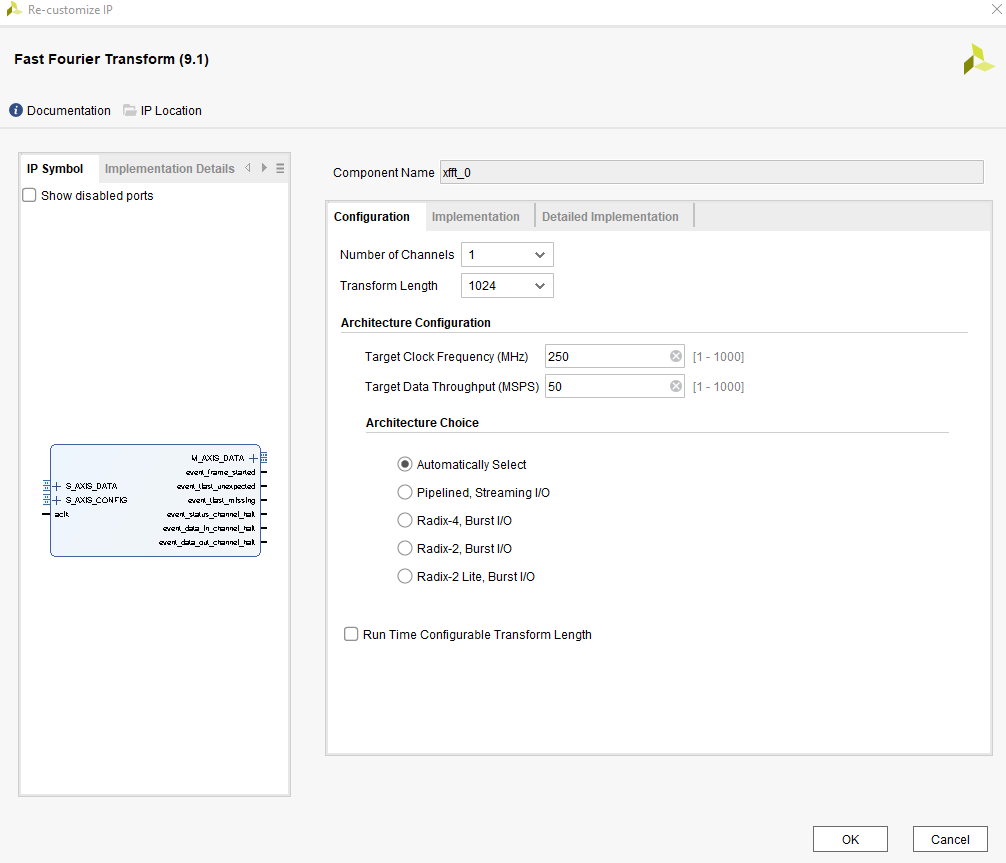
\includegraphics[width=0.5\textwidth]{image/fft_config.png}
	\caption{Временная диаграмма работы интерфейса AXI4-Stream}
	\label{fft_config}
\end{figure}
	
\begin{figure}[h]
	\centering
	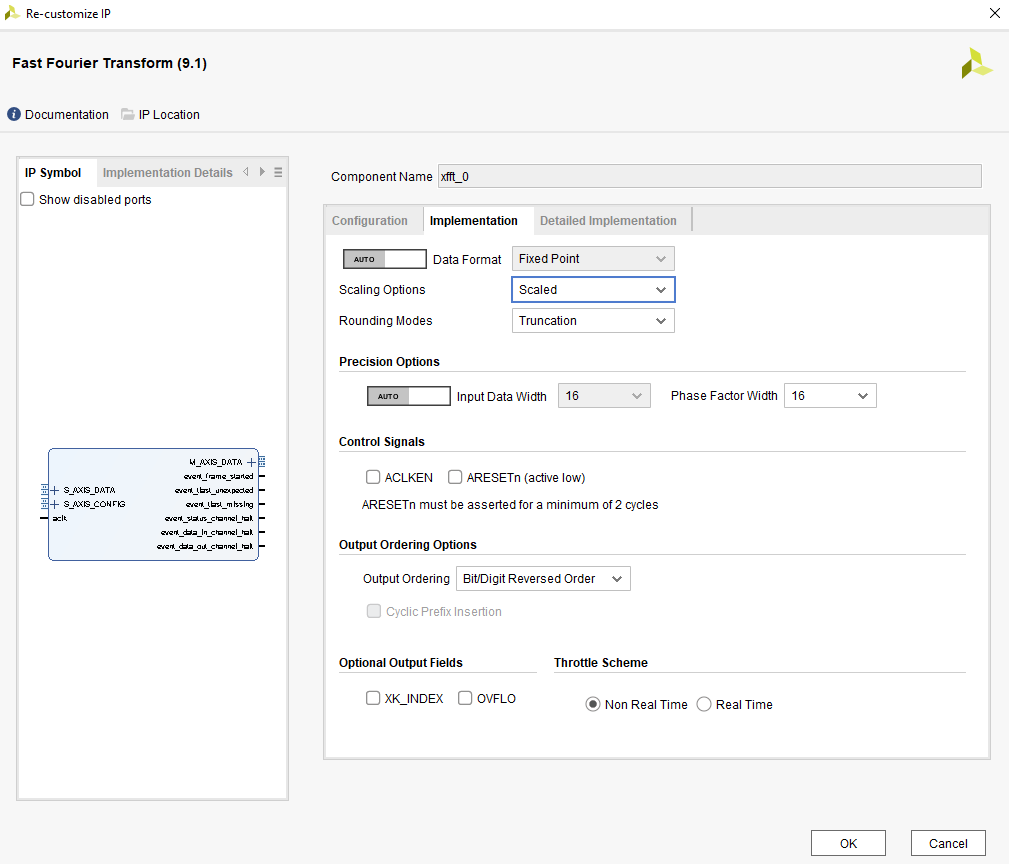
\includegraphics[width=0.5\textwidth]{image/fft_implemetation.png}
	\caption{Временная диаграмма работы интерфейса AXI4-Stream}
	\label{fft_implemetation}
\end{figure}
	
\begin{figure}[h]
	\centering
	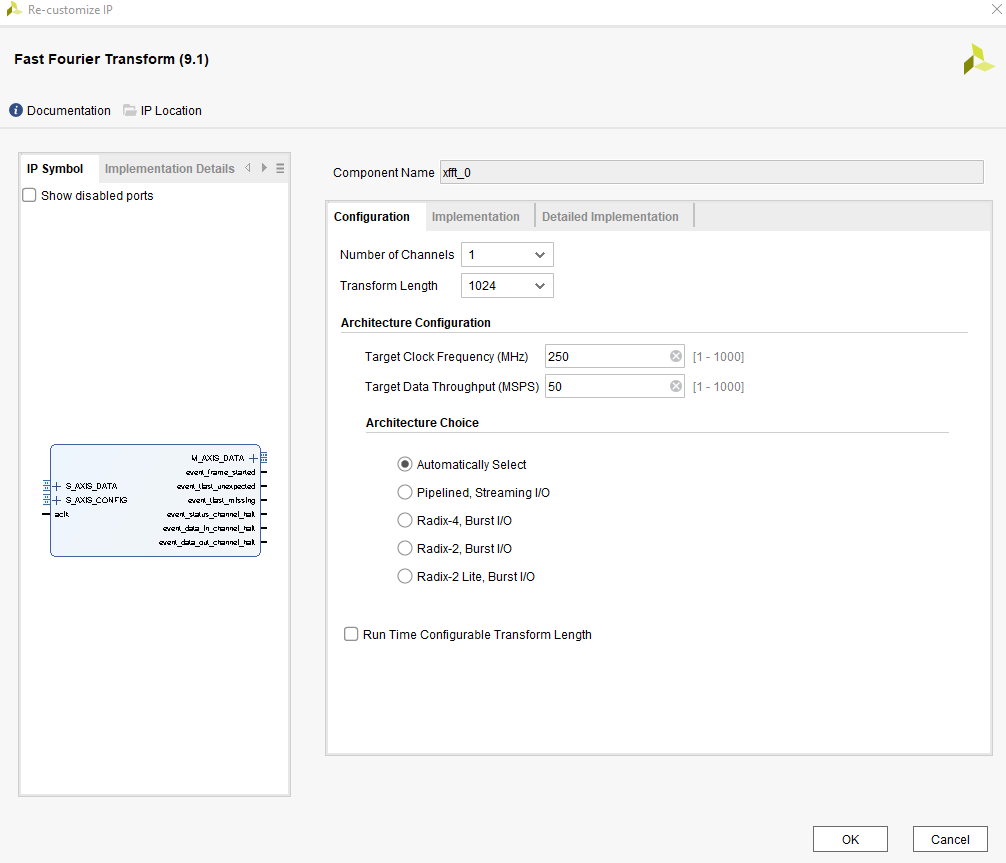
\includegraphics[width=0.5\textwidth]{image/fft_config.png}
	\caption{Временная диаграмма работы интерфейса AXI4-Stream}
	\label{fft_detailed_implem}
\end{figure}
	
\section{Сигнал с линейной-частотной модуляцией}

Сигнал с линейной-частотной модуляцией определяется по следующей формуле:
\begin{equation}	
	s(t) = rect(\frac{t}{T}) \cdot \cos(2 \cdot \pi \cdot f_0 \cdot t + j \cdot \pi \cdot K \cdot t^{2}),
\end{equation}

где t - время в секундах, K-скорость изменения частоты во времени, T - длительность импульса, rect() - прямоугольное окно, \(f_0\) - несущая частота.

После прохождения через квадратурный демодулятор получаем следующий комплексный сигнал:

\begin{equation}	
	g(t) = rect(\frac{t}{T}) \cdot \exp(j \cdot \pi \cdot K \cdot t^{2})
\end{equation}

Действительная часть называется квадратурной
составляющей ЛЧМ-сигнал, и обозначается как \(Q(t)\), а мнимая 
синфазной составляющей ЛЧМ-сигнала, и обозначается как \(I(t)\):

\begin{equation}	
	Q(t) = rect(\frac{t}{T}) \cdot \cos(\pi \cdot K \cdot t^{2}),
\end{equation}

\begin{equation}	
	I(t) = rect(\frac{t}{T}) \cdot \sin(\pi \cdot K \cdot t^{2}).
\end{equation}

Важнейшими параметрами ЛЧМ-сигнала являются:

\begin{enumerate}
	\item Девиация частоты: 
\begin{equation}
	BW = |K| \cdot T, 
\end{equation}
измеряется в Гц.
	\item База: 
\begin{equation}
	B = |K| \cdot T^2, 
\end{equation}
безразмерная величина.
\end{enumerate}

Рассмотрим конкретный пример демодулированного ЛЧМ-сигнала. Пусть он имеет следующие параметры: частота дискретизации \(F_{D}\) = 1000 МГц, девиация частоты \(BW\) = 400 МГц, длительность сигнала \(T\) = 4 мкс. На рисунке ~\ref{fig:chirp_q} представлена квадратурная составляющая ЛЧМ-сигнала с приведёнными выше параметрами, а на рисунке ~\ref{fig:chirp_i} представлена синфазная составляющая ЛЧМ-сигнала с приведёнными выше параметрами.

\begin{figure}[h]
    \centering
    \noindent
    \begin{tikzpicture}
        \begin{axis}
            [
            RCS Plot,
            title={},
            height=0.4\textwidth,
            xlabel={Время, мкс},
            ylabel={Амплитуда, отсчётов},
            legend pos = south east
            ]
            \addplot table {Synopsis/data/third-party/lfm_im.dat};
            \addlegendentry{Q(t)};
            \addplot table {Synopsis/data/third-party/lfm_re.dat};
            \addlegendentry{I(t)};
        \end{axis}
    \end{tikzpicture}
    \caption{Квадратурная составляющая ЛЧМ сигнала}
    \label{fig:chirp_q}
\end{figure}

\begin{figure}[h]
    \centering
    \noindent
    \begin{tikzpicture}
        \begin{axis}
            [
            RCS Plot,
            title={},
            height=0.4\textwidth,
            xlabel={Время, мкс},
            ylabel={Амплитуда, отсчётов},
            legend pos = south east
            ]
            \addplot table {Synopsis/data/third-party/lfm_shift_im.dat};
            \addlegendentry{Q(t)};
            \addplot table {Synopsis/data/third-party/lfm_shift_re.dat};
            \addlegendentry{I(t)};
        \end{axis}
    \end{tikzpicture}
    \caption{Квадратурная составляющая ЛЧМ сигнала}
    \label{fig:chirp_q}
\end{figure}

\begin{figure}[h]
    \centering
    \noindent
    \begin{tikzpicture}
        \begin{axis}
            [
            RCS Plot,
            title={},
            height=0.4\textwidth,
            xlabel={Время, мкс},
            ylabel={Амплитуда, отсчётов},
            legend pos = south east
            ]
            \addplot table {Synopsis/data/third-party/lfm_shift_noise_im.dat};
            \addlegendentry{Q(t)};
            \addplot table {Synopsis/data/third-party/lfm_shift_noise_re.dat};
            \addlegendentry{I(t)};
        \end{axis}
    \end{tikzpicture}
    \caption{Квадратурная составляющая ЛЧМ сигнала}
    \label{fig:chirp_q}
\end{figure}

\begin{figure}[h]
    \centering
    \noindent
    \begin{tikzpicture}
        \begin{axis}
            [
            RCS Plot,
            title={},
            height=0.4\textwidth,
            xlabel={Время, мкс},
            ylabel={Амплитуда, отсчётов},
            legend pos = south east
            ]
            \addplot table {Synopsis/data/third-party/correl_re.dat};
            \addlegendentry{I(t)};
			\addplot table {Synopsis/data/third-party/correl_im.dat};
            \addlegendentry{I(t)};
        \end{axis}
    \end{tikzpicture}
    \caption{Синфазная составляющая ЛЧМ сигнала}
    \label{fig:chirp_i}
\end{figure}


\begin{figure}[h]
	\centering
	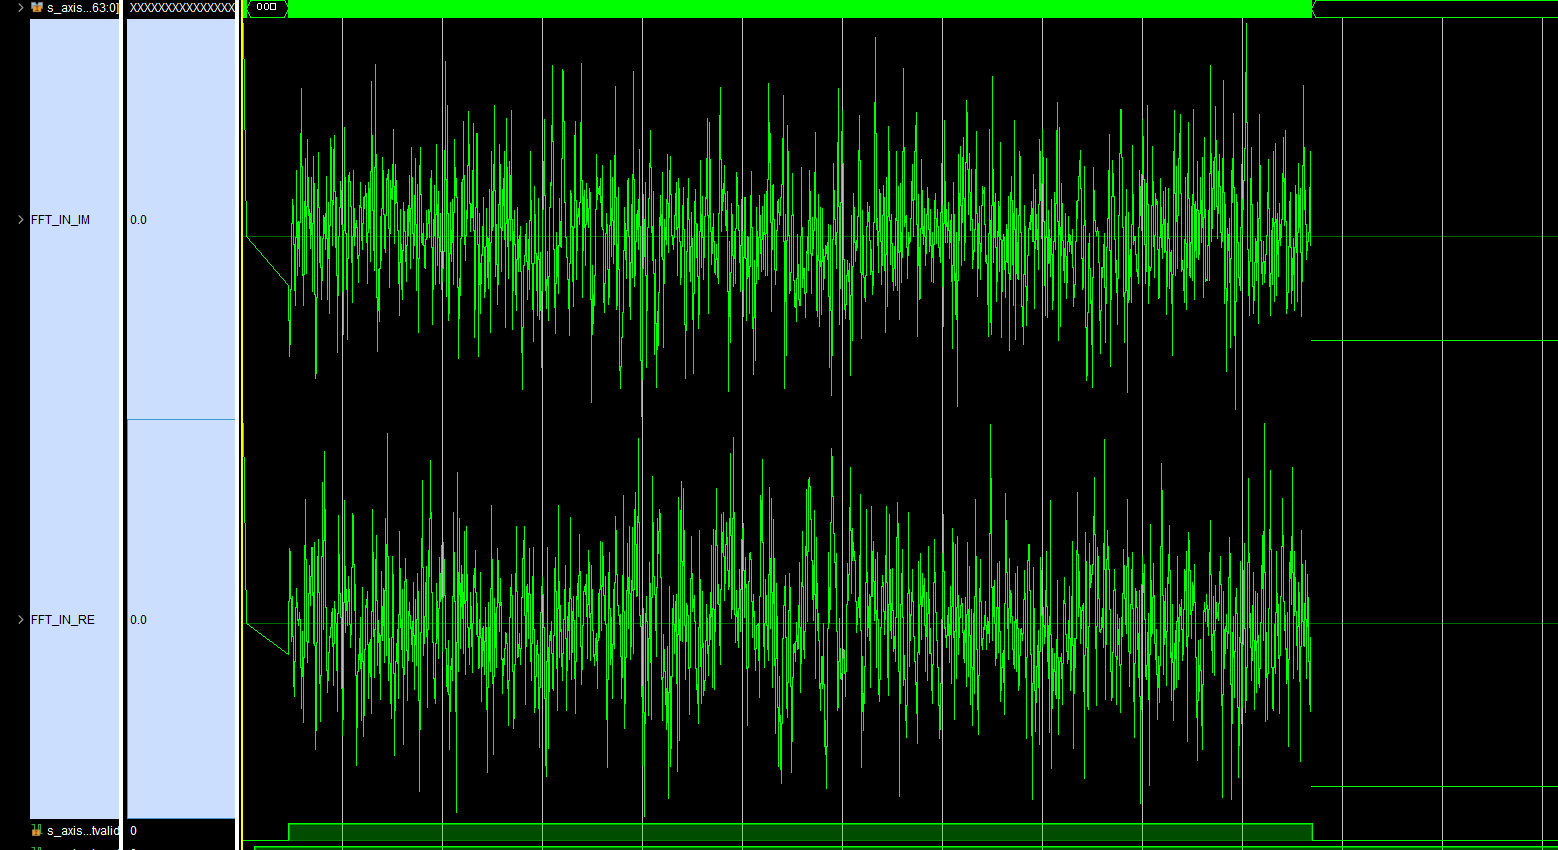
\includegraphics[width=0.5\textwidth]{image/lfm_with_noise.png}
	\caption{Временная диаграмма работы интерфейса AXI4-Stream}
	\label{fft_result}
\end{figure}
	
\begin{figure}[h]
	\centering
	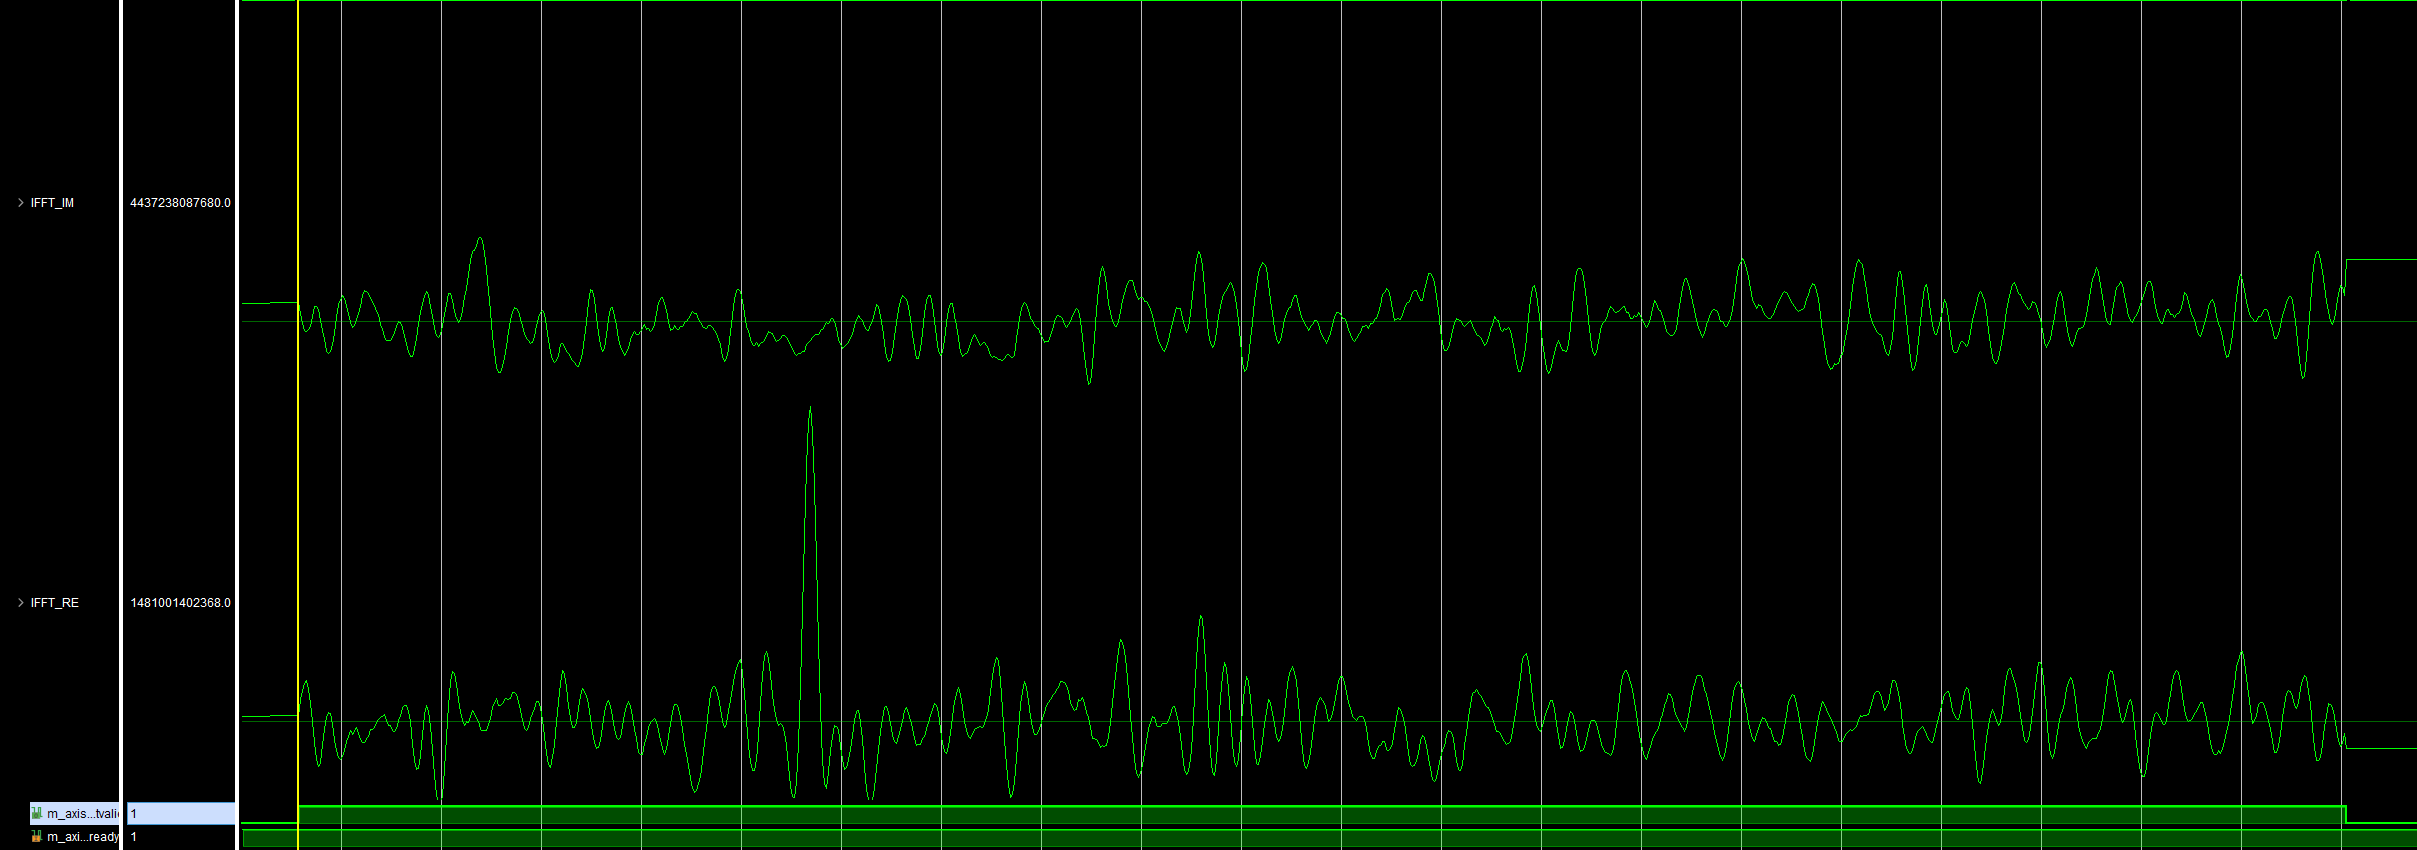
\includegraphics[width=0.5\textwidth]{image/correl_with_noise.png}
	\caption{Временная диаграмма работы интерфейса AXI4-Stream}
	\label{fft_detailed_implem}
\end{figure}

\section{Практическая часть}


